\documentclass{article}

%%%%%%%%%%%%%%%%%%%%%%%%%%%%%%%%%%%%%%%%%%%%%%%%%%%%%%%%
% Packages
%%%%%%%%%%%%%%%%%%%%%%%%%%%%%%%%%%%%%%%%%%%%%%%%%%%%%%%%

%\usepackage[utf8]{inputenc} % for overleaf/PLM
\usepackage[latin1]{inputenc} % averil local
\usepackage[T1]{fontenc} % hyphenation
\usepackage{fullpage} % DO NOT USE IN BEAMER
\usepackage[british,UKenglish,USenglish,american]{babel}
%\usepackage{appendix}
\usepackage{amssymb,amsmath,amsthm,enumerate}
\usepackage{mathtools} % coloneqq
%\usepackage{easybmat}
\usepackage{enumitem}
%\usepackage{tikz}
%\usepackage{caption}
\usepackage{float} % [H]
%\usepackage{bbold}
\usepackage{xcolor}
\usepackage{stmaryrd} % ll/rr brackets
%\usepackage[tworuled,vlined,nofillcomment]{algorithm2e}
\usepackage[ruled,vlined]{algorithm2e}
\usepackage{cases} % numbered lines in cases (numcases and subnumcases)
\usepackage{cleveref} % \cref. 

%%%%%%%%%%%%%%%%%%%%%%%%%%%%%%%%%%%%%%%%%%%%%%%%%%%%%%%%
% Format
%%%%%%%%%%%%%%%%%%%%%%%%%%%%%%%%%%%%%%%%%%%%%%%%%%%%%%%%

\title{Numerical methods for plasma sheaths}
\author{
	Valentin Ayot\footnote{Institut de Math�matiques, CNRS, UMR 5251, Universit� de Bordeaux, F-33405 Talence, France. \texttt{valentin.ayot@u-bordeaux.fr}}, 
	 \ Averil Prost\footnote{INSA de Rouen, LMI (EA 3226 - FR CNRS 3335), 685 Avenue de l'Universit�, 76801 St Etienne du Rouvray cedex, France. \texttt{averil.prost@insa-rouen.fr}}, 
	 \ Christian Tayou-Fotso\footnote{Labo. J. A. Dieudonn�, UMR 6621, Universit� Nice-Sophia Antipolis, Parc Valrose, F-06108 Nice cedex 02, France. \texttt{christian.tayou-fotso@unice.fr}}.
 } 
\date{}

\SetKwRepeat{Do}{do}{while} % for algorithm2e package, add do-while

% set dashes instead of bullets for item lists
\setlist[itemize,1]{label=$-$}
\setlist[itemize,2]{label=$-$}
\setlist[itemize,3]{label=$-$}

% remove unnecessary formatting of clever references
\crefdefaultlabelformat{(#2#1#3)}
\crefname{equation}{}{}

%%%%%%%%%%%%%%%%%%%%%%%%%%%%%%%%%%%%%%%%%%%%%%%%%%%%%%%%
% Theorems
%%%%%%%%%%%%%%%%%%%%%%%%%%%%%%%%%%%%%%%%%%%%%%%%%%%%%%%%

\newtheorem{proposition}{Proposition}[section]
\newtheorem{definition}{Definition}[section]
\newtheorem{theoreme}{Theorem}[section]
\newtheorem{remarque}{Remark}[section]
\newtheorem{lemme}{Lemma}[section]
\numberwithin{equation}{section}

%%%%%%%%%%%%%%%%%%%%%%%%%%%%%%%%%%%%%%%%%%%%%%%%%%%%%%%%
% Commands
%%%%%%%%%%%%%%%%%%%%%%%%%%%%%%%%%%%%%%%%%%%%%%%%%%%%%%%%

\newcommand{\N}{\mathbb{N}}
\newcommand{\Z}{\mathbb{Z}}
\newcommand{\R}{\mathbb{R}}
\newcommand{\lp}{\left(}
\newcommand{\rp}{\right)}
\newcommand{\tran}[1]{\prescript{t}{}{#1}}
\newcommand{\vol}{\textup{Vol}}
\newcommand{\red}{\textcolor{red}}
\newcommand{\blue}{\textcolor{blue}}

\newcommand{\todo}[1]{{\color{red}\textbf{#1}}}
\newcommand{\vv}[1]{\begin{pmatrix} #1 \end{pmatrix}} % vector

%\renewcommand\appendixpagename{Appendix}
%\renewcommand\appendixtocname{Appendix}
\renewcommand{\qedsymbol}{$\blacksquare$}

%%%%%%%%%%%%%%%%%%%%%%%%%%%%%%%%%%%%%%%%%%%%%%%%%%%%%%%%
%%%%%%%%%%%%%%%%%%%%%%%%%%%%%%%%%%%%%%%%%%%%%%%%%%%%%%%%
%%%%%%%%%%%%%%%%%%%%%%%%%%%%%%%%%%%%%%%%%%%%%%%%%%%%%%%%

\begin{document}
	
\maketitle

\begin{abstract}
This article is a report of the project achieved during the CEMRACS 2022.
\end{abstract}

%% Plan
% 1 : Model : 
% 	- motivation, model, difficulties
%	- boundary conditions
%	- symmetries
% 2 : Numerical methods
% 3 : Numerical results : DO WE HAVE SHEATHS????

\section{Plasma sheaths}

\paragraph{The model}

Let $f_i : \R^+ \times [-1,1]\times \R \mapsto \R$ denote the ion density, $f_e : \R^+ \times [-1,1]\times \R \mapsto \R$ denote the electron density, and $\varphi : \R^+ \times [-1,1] \mapsto \R$ denote the electric potential. We define the densities $n_{i,e}$ and currents $J_{i,e}$ as
\begin{align}\label{eq:def_ni_ne}
	n_{i,e} (t,x) \coloneqq \int_{v\in\R} f_{i,e} (t,x,v) dv, \quad J_{i,e} (t,x) \coloneqq \int_{v\in\R} v f_{i,e} (t,x,v) dv.
\end{align}
In the sequel, we will denote $n (t,x) \coloneqq n_i (t,x) - n_e(t,x)$, and $J(t,x) \coloneqq J_i(t,x) - J_e(t,x)$.
Let $\nu \geqslant 0$ be the ionization frequency, $\mu \coloneqq \frac{m_e}{m_i} > 0$ be the mass ratio between the electrons and the ions, and $\lambda>0$ be the Debye length.

We consider the following unstationary model: determine $f_{i,e} = f_{i,e}(t,x,v)$ and $\varphi = \varphi(t,x)$ such that
\begin{subnumcases}{\label{eq:unsta_model}}
	\partial_t f_i + v \partial_x f_i - \partial_x \varphi \, \partial_v f_i = \nu f_e \hfill (t,x,v) \in \R_{*}^{+} \times ]-1,1[ \times \R, \\
	\partial_t f_i + v \partial_x f_e + \frac{\partial_x \varphi }{\mu}\, \partial_v f_e = 0 \quad\quad\hfill (t,x,v) \in \R_{*}^{+} \times ]-1,1[ \times \R,\\
	- \lambda^2 \partial^2_{xx} \varphi = n (t,x) \hfill (t,x) \in \R^{+} \times ]-1,1[.
\end{subnumcases}

To reduce the notations, we will use $f_s$, $s\in\{i,e\}$ to denote both the electronic and ionic distribution, and the speed coefficients $c_s$ and source terms $S_s$ defined as
\begin{align*}
	c_i \coloneqq 1, \quad c_e \coloneqq -\frac{1}{\mu}, \quad S_i \coloneqq \nu f_e, \quad S_e \coloneqq 0.
\end{align*}

This model is supplemented with
%\begin{align}
%		f_{s}(0,x,v) &\coloneqq f_{s}^0(x,v) && (x,v) \in ]-1,1[ \times \R \quad \text{Initial conditions,} \label{eq:init} \\
%		\varphi(t,0) &\coloneqq 0  && t \in \R^+ \quad \text{Reference potential,} \label{eq:phi_nul_0} \\
%		\pm \partial_x \varphi(t,\pm 1) &\coloneqq C(t) && t \in \R^+ \quad \text{Neumann boundary conditions,} \label{eq:phi_bc_C} \\
%		f_{s}(t,x=\pm 1,\pm v < 0) &\coloneqq 0 && t \in \R^+_* \quad \text{Non-emitting boundary conditions.} \label{eq:fie_bc}
%\end{align}
\begin{subnumcases}{}
	f_{s}(0,x,v) \coloneqq f_{s}^0(x,v)  \quad\quad (x,v) \in ]-1,1[ \times \R  & Initial conditions, \label{eq:init} \\
	\varphi(t,0) \coloneqq 0 \hfill t \in \R^+ & Reference potential, \label{eq:phi_nul_0} \\
	\pm \partial_x \varphi(t,\pm 1) \coloneqq C(t) \hfill t \in \R^+ & Neumann boundary conditions, \label{eq:phi_bc_C} \\
	f_{s}(t,x=\pm 1,\pm v < 0) \coloneqq 0  \hfill t \in \R^+_* & Non-emitting boundary conditions. \label{eq:fie_bc}
\end{subnumcases}

The Neumann boundary condition $t \to C(t)$ will be precised in \cref{subsec:poisson_bc}.

We may reformulate the model using the electric field $(t,x) \to E(t,x) \coloneqq - \partial_x \varphi(t,x)$. This variable satisfies the first-order equation 
\begin{align}\label{eq:Poisson_E}
	\lambda^2 \partial_x E (t,x) = n (t,x), \quad E(t,\pm 1) = \mp C(t).  
\end{align}

\todo{Big structure assumption : 
In the sequel, we make the following assumptions:
\begin{itemize}
\item There exists a solution $(f_i, f_e, \varphi)$ of the system \cref{eq:unsta_model}.
\item The function $\varphi$ satisfies the symmetry $\varphi(x) = \varphi(-x)$.
\item The function $n : [-1,1] \mapsto \R$ is nonnegative. 
\item The function $\varphi$ is of class $\mathcal{C}^2(\R^+_* \times ]-1,1[) \cap \mathcal{C}(\R^+ \times [-1,1])$.
\end{itemize}
Notice that $n \geqslant 0$ implies that $\varphi$ is concave. Owing to the smoothness of $\varphi$ and the symmetry assumption, we also have $\partial_x \varphi(t,0)=0$, and $\varphi$ is nonpositive.
}

%\section{Boundary conditions}
%\subsection{Boundary condition for the Poisson equation}\label{subsec:poisson_bc}
%
%\todo{To clarify:
%\begin{itemize}
%\item Either we consider / assume that $\varphi$ will be smooth, and the symmetry gives $E(t,0)=-\varphi_x \varphi(t,0) = 0$, way simpler.
%\item Or we consider that $\varphi$ is not derivable at $x=0$, i.e. $E$ is not continuous at $x=0$ (ex. $\nu=0$ but $f_i(t,0,0) \neq 0$ ?), and in this case, not enough regularity to perform the computations correctly...
%\end{itemize}
%}
%
%Here, we derive the boundary condition $t \to C(t)$ for $\varphi$. We assume that $\varphi \in C^{2,3}(\R^+_* \times ]-1,1[)$.
%
%First, we derive with respect to time the Poisson equation 
%\begin{align*}
%	- \partial_t (\lambda^2\partial_{xx}^2 \varphi) = \partial_t n, 	
%\end{align*}
%and considering the difference between the $v$-integration of the Vlasov equations gives 
%\begin{align*}
%	\partial_t n = \partial_t (n_i - n_e) = \nu n_e - \partial_x (J_i - J_e) = \nu n_e - \partial_x J,
%\end{align*}
%so that, using $E=-\partial_x \varphi$, we get 
%\begin{align*}
%	\partial_x (\lambda^2\partial_t E + J) = \nu n_e, \quad \forall x\in ]-1, 1[. 	
%\end{align*}
%
%Integrating now in space leads to 
%\begin{align}\label{eq:ampere_integ}
%	\lambda^2\partial_t E(t, 1) + J(t, 1) = \lambda^2\partial_t E(t, -1) + J(t, -1) +\nu \int_{-1}^1 n_e (t, x) dx,  
%\end{align}
%and using the symmetries $E(t,x)=-E(t, -x)$ and  $J(t,x)=-J(t, -x)$, it comes 
%\begin{align}\label{eq:ampere_bc}
%	\lambda^2\partial_t E(t, \pm 1) + J(t, \pm 1)  = \pm \frac{\nu}{2} \int_{-1}^1 n_e (t, x)dx.
%\end{align}
%Integrating in time yields the value of $C$:
%\begin{align}\label{eq:ampere_bc_phi}
%%	\partial_x \varphi(t, 1) =\partial_x \varphi(0, 1) +\frac{1}{\lambda^2}\int_0^t (J_i-J_e)(s, 1)ds - \frac{\nu}{2\lambda^2}\int_0^t  \int_{-1}^1 \rho_e(s, x)dx ds \equiv C(t). 
%%	- \lambda^2 \partial_x \varphi(t, 1) + \lambda^2 \partial_x \varphi (0, 1) + \int_0^t J (s, 1) ds &=  \frac{\nu}{2}\int_0^t  \int_{-1}^1 n_e (s, x) dx ds \equiv C(t). \\
%	\partial_x \varphi(t, 1) &= \partial_x \varphi (0, 1) + \frac{1}{\lambda^2} \int_0^t J (s, 1) ds - \frac{\nu}{2 \lambda^2}\int_0^t  \int_{-1}^1 n_e (s, x) dx ds \equiv C(t). 
%\end{align}

\section{Numerical methods}



\subsection{Poisson equation}

\todo{First case: we use symmetry assumption}

Owing to the symmetry assumption, we have $E(t,x) = -E(t,-x)$, thus $E(t,0) = 0$. Then, integrating the Poisson problem \cref{eq:Poisson_E} over $[0,x]$ yields
\begin{align}\label{eq:integral_representation_E_sym}
	E(t,x) = 0 + \int_0^x n(t,y) dy = \int_0^x \int_{v\in\R} [f_i(t,y,v) - f_e(t,y,v)] dv dy.
\end{align}
This expression may be approximated by quadrature formulas.

\todo{Second case: we use natural boundary condition}

The boundary condition deduced in \cref{subsec:poisson_bc} yields $E(t,\pm 1) = \mp C(t)$. We split the domain into its positive and negative part, and consider the exact representation
\begin{align}\label{eq:integral_representation_E_naturalbc}
	E(t,x) = 
	\begin{cases}
	E(t,\phantom{-}1) - \int_{x\phantom{-}}^{1} n(t,y) dy = - C(t) - \int_{x\phantom{-}}^1 \int_{v\in\R} [f_i(t,y,v) - f_e(t,y,v)] dv dy & x \in [0,1] \\
	E(t,-1) + \int_{-1}^x n(t,y) dy = \phantom{-}C(t) + \int_{-1}^x \int_{v\in\R} [f_i(t,y,v) - f_e(t,y,v)] dv dy & x \in [-1,0[ 
	\end{cases}
\end{align}
This expression may be approximated by quadrature formulas. Note that here, the numerical approximation may "jump" at $x=0$.

\todo{End cases.}


\subsection{Finite Differences (FD)}

Define a numerical computation domain $\Omega \coloneqq [-1,1] \times [-\overline{V},\overline{V}]$, with a large enough maximum speed $\overline{V}$. Let $(x_j, v_k)^{j\in\llbracket0,J\rrbracket}_{k\in\llbracket0,K\rrbracket}$ be a cartesian grid of $\Omega$ of step $(\Delta x, \Delta v)$. We discretize the advection equations on the subgrid $(x_j, v_k)^{j\in\llbracket1,J-1\rrbracket}_{k\in\llbracket1,K-1\rrbracket}$ by an explicit Euler scheme in time, and the upwind scheme in space:
\begin{align}\label{eq:FDscheme}
	\frac{f_{s,j,k}^{n+1} - f_{s,j,k}^{n}}{\Delta t} + D^-_{j,k} f_s^n \vv{v_k\\c_s E_j^n}_{+} +D^+_{j,k} f_s^n \vv{v_k\\c_s E_j^n}_{-} = S_{s,j,k}^n,
\end{align}
where $a_+ = \max(a,0)$ and $a_{-} = \min(a,0)$ are respectively the pointwise positive and negative parts, and the decentered discrete differentials are defined as
\begin{align*}
	D^{\pm}_{j,k} f \coloneqq \pm \left(\frac{f_{j\pm 1,k} - f_{j,k}}{\Delta x}, \frac{f_{j,k\pm 1} - f_{j,k}}{\Delta v}\right).
\end{align*}

The values of $f_{s,j,k}^n$ on the boundary are taken as follows:
\begin{itemize}
\item the boundary condition \cref{eq:fie_bc} yields $f_{s,j,k}^n = 0$ whenever $x_j=-1, v_k > 0$ or $x_j=1, v_k < 0$.
\item It is considered that $\overline{V}$ is large enough to take the values on the speed boundary $v_k = \pm \overline{V}$ equal to 0.
\item The remaining values $f_{s,j,k}^n$, $x_j=-1, -\overline{V} < v_k \leqslant 0$ or $x_j=1, 0 \leqslant v_k < \overline{V}$ may be computed using the scheme \cref{eq:FDscheme}, since the sign of the speed allows to use only inner points.
\end{itemize}

With these approximations, we may compute the electric field $E$ by a quadrature approximation of the integral representation \todo{either} \cref{eq:integral_representation_E_sym} \todo{or} \cref{eq:integral_representation_E_naturalbc}.

The upwind scheme is known to be diffusive, and stable under the CFL condition 
\begin{align*}
	1 - \max_{k} |v_k| \frac{\Delta t}{\Delta x} - |c_s| \max_{j} |E^n_j| \frac{\Delta t}{\Delta v} \geqslant 0 \quad \forall s \in \{i,e\}\text{ and } n \in \llbracket1,N\rrbracket.
\end{align*}
Given $\Delta x$ and $\Delta v$, we deduce a sufficiently small value of $\Delta t$ with the bound
\begin{align*}
	\Delta t \leqslant \min\left(\frac{\Delta x}{\overline{V}}, \max(1,\mu)\frac{\Delta v}{E_{\text{max}}}\right), \quad E_{\text{max}}>0 \text{ postulated \emph{a priori}.}
\end{align*}

\subsection{Semi-Lagrangian (SL)}

We use a splitting method in time. The full model \cref{eq:unsta_model} is decomposed in elementary operators, namely
\begin{itemize}
\item The 1D advection operators along dimensions $x$ and $v$, given by the flows of $\partial_t f + v \partial_x f = 0$ and $\partial_t f + c_s E \partial_v f = 0$, with $c_s \in \{1, -\frac{1}{\mu}\}$.
\item The resolution of the Poisson problem.
\end{itemize}
We use Strang splitting to reach order 2 in time. More precisely, the algorithm is given by

%\todo{EITHER ALGO FORMULATION}
%
%\begin{algorithm}[H]
%	\DontPrintSemicolon
%	\SetAlgoLined
%	Let $f_{i,e}^0$ be given.\;
%	Solve the Poisson problem for $E^0$. \;
%	\For{$n \in \llbracket1,N\rrbracket$}{
%		Solve the homogeneous advection in variable $x$ for $f_{i,e}^*$ on time step $\Delta t/2$.\;
%		Solve the Poisson problem for $E^{n,*}$.\;
%		Solve the pointwise ODE $\partial_t f_i = \nu f_e^{*}$ for $f_i^{**}$ on time step $\Delta t/2$.\;
%		Solve the advection in variable $v$ for $f_{i,e}^{***}$ on time step $\Delta t$.\;
%		Solve the pointwise ODE $\partial_t f_i = \nu f_e^{***}$ for $f_i^{****}$ on time step $\Delta t/2$.\;
%		Solve the Poisson problem for $E^{n+1}$.\;
%		Solve the homogeneous advection in variable $x$ for $f_{i,e}^{n+1}$ on time step $\Delta t/2$.\;
%	}
%	\caption{Semi-Lagrangian scheme}
%\end{algorithm}
%
%\todo{OR EQUATION FORMULATION}

%Following \todo{ref Michel ?}, we decompose the full model \cref{eq:unsta_model} in 	
%\begin{align*}
%	\mathcal{A}_{s,x}^{\Delta t / 2} \circ \mathcal{P}^{\Delta t / 2} \circ \mathcal{A}_{s,v}^{\Delta t} \circ \mathcal{P}^{\Delta t / 2} \circ \mathcal{A}_{s,x}^{\Delta t / 2} 
%\end{align*}
\begin{align*}
	\frac{\Delta t}{2} \quad\quad&
	\begin{cases}
		\partial_t f_s + v \partial_x f_s = 0 & \text{Linear advection along $x$,} \\
		\lambda^2 \partial_x E = n_i - n_e & \text{Poisson problem,} \\
	\end{cases} \\
%%%
	\frac{\Delta t}{2} \quad\quad&
	\partial_t f_i = \nu f_e \quad\quad\quad\quad\quad \text{Source term,} \\
%%%
	\Delta t \quad\quad&
	\partial_t f_s + c_s E \partial_v f_s = 0 \quad \text{Linear advection along $v$,} \\
%%%
	\frac{\Delta t}{2} \quad\quad&
	\partial_t f_i = \nu f_e \quad\quad\quad\quad\quad \text{Source term,} \\
%%%
	\frac{\Delta t}{2} \quad\quad&
	\begin{cases}
		\lambda^2 \partial_x E = n_i - n_e & \text{Poisson problem,}\\
		\partial_t f_s + v \partial_x f_s = 0 & \text{Linear advection along $x$.}
	\end{cases} 
\end{align*}

%\todo{END EITHER OR.}

Notice that each advection is at constant speed with respect to the advection variable. This allows for the use of elementary 1D solvers. \todo{We now describe the treatment of the boundaries.} 
%In order to describe the algorithm completely, we need to give the detail of the resolution of the Poisson problem. 


\paragraph{Numerical treatment of the boundaries}

The full model \cref{eq:unsta_model} includes multi-dimensional advection equations for $f_{i,e}$, supplemented with well-placed boundary conditions \cref{eq:fie_bc}. However, the main algorithm uses a splitting method that relies on 1D advection solvers. Therefore, we may first focus on the elementary advection equation with constant speed $a>0$
\begin{align*}
	\partial_t f (t,x) + a \partial_x f(t,x) = 0, \quad f(t,-1) = 0, \quad \forall (t,x) \in \R^+_* \times ]-1,1[.
\end{align*}
Let $(x_j)_{j\in\llbracket0,J\rrbracket}$ be a space mesh of step $\Delta x \coloneqq 2/J$, and $(t_n)_{n\in\llbracket 0,N \rrbracket}$ be a time mesh of step $\Delta t \coloneqq T/N$.
We follow the work of \cite{coulombelNeumannNumericalBoundary2020}, and consider a semi-Lagrangian scheme defined as
\begin{align*}
	f^{n+1}_j = \text{Lagrange interpolation}\left(f^n, x_j - a \Delta t\right) \coloneqq \sum_{k=-d}^d f^n_{j+k} L_k (x_j - a \Delta t).
\end{align*}
The stencil of the Lagrange interpolation uses $2d + 2$ points, where $d\in\N$.
%The Lagrange interpolation will use a centered stencil of $2d+2$ points, where $d\in\N$. 
The boundaries are treated as follow:
\begin{itemize}
\item the \emph{inflow} side, corresponding to $x=-1$, relies on the analytical solution $f(t,x) = 0$ $\forall x \leqslant a t$. Whenever the scheme needs a value $f^n_j$ with $j < 0$, it may be exactly taken equal to 0.
\item in the case $d>0$, the Lagrange stencil may also need \emph{outflow} values $f^n_{j}$ with $j>J$. Such values may be determined by polynomial extrapolation. Let $k_b \in \N$, and let $p$ be the unique polynomial of order $k_b$ interpolating $(x_j, f^n_j)$ for $j\in \llbracket J-kb,J\rrbracket$. The \emph{outflow ghost points} will be defined by $f^n_j \coloneqq p(-1 + j \Delta x)$ $\forall j > N$. 
\end{itemize}

%\subsection{Fixed-point (FP)}
%
%This algorithm is heavily inspired from the fixed-point procedure developped in \cite{badsiStableFixedPoint2021} for a collisional model.
%We focus on the equilibrium state $(f_i, f_e, \varphi)$ solving the stationary system
%%\begin{align}\label{eq:sta_model}
%%	\begin{cases}
%%		v \partial_x f_i (x,v) - \partial_x \varphi(x) \partial_v f_i(x,v) = \nu f_e (x,v) & (x,v) \in ]-1,1[ \times \R, \\
%%		v \partial_x f_e (x,v) + \frac{1}{\mu}\partial_x \varphi(x) \partial_v f_e(x,v) = 0 & (x,v) \in ]-1,1[ \times \R,\\
%%		- \lambda^2 \partial^2_{xx} \varphi (x) = n (x) & x \in ]-1,1[.
%%	\end{cases}
%%\end{align}
%\begin{subnumcases}{\label{eq:sta_model}}
%		v \partial_x f_i (x,v) - \partial_x \varphi(x) \,\partial_v f_i(x,v) = \nu f_e (x,v) \quad\quad (x,v) \in ]-1,1[ \times \R, \label{eq:sta_model_fi} \\
%		v \partial_x f_e (x,v) + \frac{\partial_x \varphi(x)}{\mu} \partial_v f_e(x,v) = 0 \hfill (x,v) \in ]-1,1[ \times \R, \label{eq:sta_model_fe}\\
%		- \lambda^2 \partial^2_{xx} \varphi (x) = n (x) \hfill x \in ]-1,1[. \label{eq:sta_model_phi}
%\end{subnumcases}
%
%To be consistent with the evolutionary model \cref{eq:unsta_model}, the following boundary conditions are considered:
%\begin{subnumcases}{}
%		\varphi(0) \coloneqq 0  & Reference potential, \\
%		\pm \partial_x \varphi(\pm 1) \coloneqq C & Neumann boundary conditions, \\
%		f_{s}(x=\pm 1,\pm v < 0) \coloneqq 0 & Non-emitting boundary conditions.
%\end{subnumcases}
%However, the problem lack some additional information to be well-posed. Indeed, the advection equation \cref{eq:sta_model_fe} implies that $f_e$ is constant along its characteristic lines, given by the level lines of the infinitesimal energy $\mathcal{L}_e (x,v) \coloneqq \frac{v^2}{2} - \frac{\varphi}{\mu}$. According to the structure of $\varphi$, these curves are closed, and may not cross the boundary $x=\pm 1$ (see \cref{fig:characteristics}). We give a value to these lines by enforcing
%\begin{align}\label{eq:sta_feb}
%	f_e(0,v) = f_{e,b} (v), \quad \forall v \leqslant 0. 
%\end{align}
%\todo{Accorder les notations entre Mehdi, Nicolas, Ana�s, Michel, Yann, le pape et Averil.}
%
%\begin{figure}
%	\centering
%	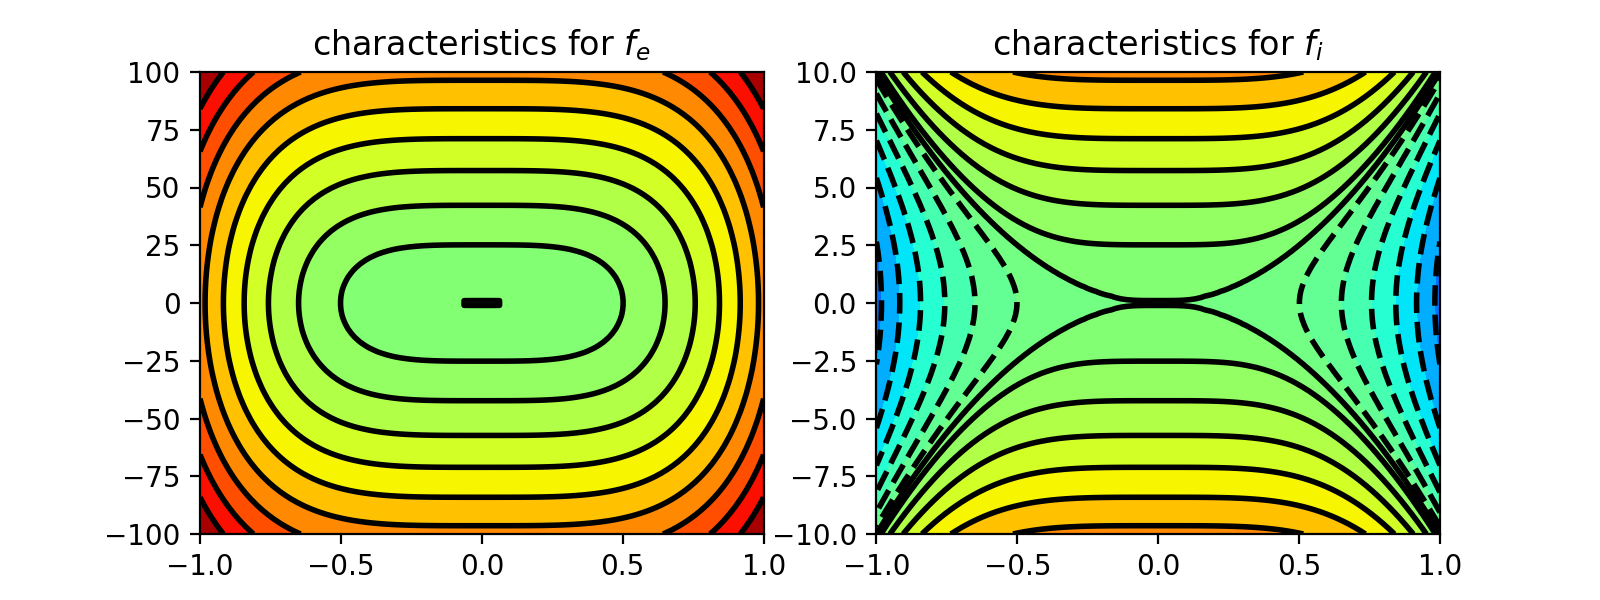
\includegraphics[width=0.9\linewidth]{images/characteristics}
%	\caption{Typical structure of the characteristic lines in the plan $(x,v)$.}
%	\label{fig:characteristics}
%\end{figure}
%
%Let us describe the fixed-point steps. Suppose that a candidate $\varphi^k$ is given. Then:
%\begin{enumerate}
%\item We may deduce the characteristic lines for the equations \cref{eq:sta_model_fi,eq:sta_model_fe}, and compute approximations $f_{i,e}^k$.
%\item By integration on $v$, we may compute $n^k \coloneqq n_i^k - n_e^k$.
%\item The next iterate $\varphi^{k+1}$ is defined as the solution of the Poisson problem \cref{eq:sta_model_phi} with source term $n^k$.
%\end{enumerate}

\section{Numerical results}
\subsection{1-species validation test case}
%\subsection{2-species results}
% Diagnostics (conservations)
% Do we observe sheaths? 
\subsection{Comparison between (SL) and (FD)}
%\subsection{Comparison between (SL) and (FP)}
%% plugging one into the other and the other way around

\bibliographystyle{alpha}
\bibliography{CEMRACS.bib}

\end{document}